% Implicit and explicit inference, as two vertical chains from the prior to the data.
% One source, two renders on the same scale: \stage=1 gives implicit.svg, \stage=2 explicit.svg.
% The titles are on the slide, above each figure.
% Compile: pdflatex -jobname=implicit "\def\stage{1}% Implicit and explicit inference, as two vertical chains from the prior to the data.
% One source, two renders on the same scale: \stage=1 gives implicit.svg, \stage=2 explicit.svg.
% The titles are on the slide, above each figure.
% Compile: pdflatex -jobname=implicit "\def\stage{1}% Implicit and explicit inference, as two vertical chains from the prior to the data.
% One source, two renders on the same scale: \stage=1 gives implicit.svg, \stage=2 explicit.svg.
% The titles are on the slide, above each figure.
% Compile: pdflatex -jobname=implicit "\def\stage{1}% Implicit and explicit inference, as two vertical chains from the prior to the data.
% One source, two renders on the same scale: \stage=1 gives implicit.svg, \stage=2 explicit.svg.
% The titles are on the slide, above each figure.
% Compile: pdflatex -jobname=implicit "\def\stage{1}\input{implicit_explicit.tex}" (and explicit, \stage{2}), then pdftocairo -svg.
\documentclass[tikz,border=4pt]{standalone}
\usepackage{tikz}
\usepackage{amsmath}
\usepackage[T1]{fontenc}
\usetikzlibrary{arrows.meta,positioning,calc,shapes.geometric}

\providecommand{\stage}{1}

\definecolor{ink}{HTML}{2E2E2E}
\definecolor{greytx}{HTML}{7A7A7A}
\definecolor{flow}{HTML}{3B6FB6}
\definecolor{priortop}{HTML}{D8EDD2}
\definecolor{priorbot}{HTML}{8FCB7E}
\definecolor{priorrim}{HTML}{6DAF5C}
\definecolor{side}{HTML}{E4E4E4}
\definecolor{datatop}{HTML}{E3ECF7}
\definecolor{databot}{HTML}{9DBBD8}

\tikzset{
  prior/.style={circle,minimum size=1.9cm,draw=priorrim,line width=0.8pt,
                top color=priortop,bottom color=priorbot,text=ink,font=\Large},
  flowarr/.style={-{Stealth[length=3.4mm,width=2.8mm]},line width=1.5pt,draw=flow},
  data/.style={circle,minimum size=1.7cm,draw=flow,line width=0.8pt,
               top color=datatop,bottom color=databot,text=ink,font=\Large},
  card/.style={draw=ink,line width=0.9pt,rounded corners=7pt,fill=white,align=center,
               text=ink,font=\sffamily},
}

% A white 3D box: front face as a node, with a bevelled top and left side behind it.
% #1 node name, #2 position, #3 width, #4 height, #5 label
\newcommand{\simbox}[5]{%
  \node[draw=ink,line width=0.9pt,fill=white,minimum width=#3,minimum height=#4,
        align=center,text=ink,font=\sffamily\large] (#1) at #2 {#5};
  \fill[side,draw=ink,line width=0.9pt]
    (#1.north west) -- ++(-0.35,0.35) -- ($(#1.north east)+(-0.35,0.35)$) -- (#1.north east) -- cycle;
  \fill[side!70!black!40,draw=ink,line width=0.9pt]
    (#1.north west) -- ++(-0.35,0.35) -- ($(#1.south west)+(-0.35,0.35)$) -- (#1.south west) -- cycle;
}

\begin{document}
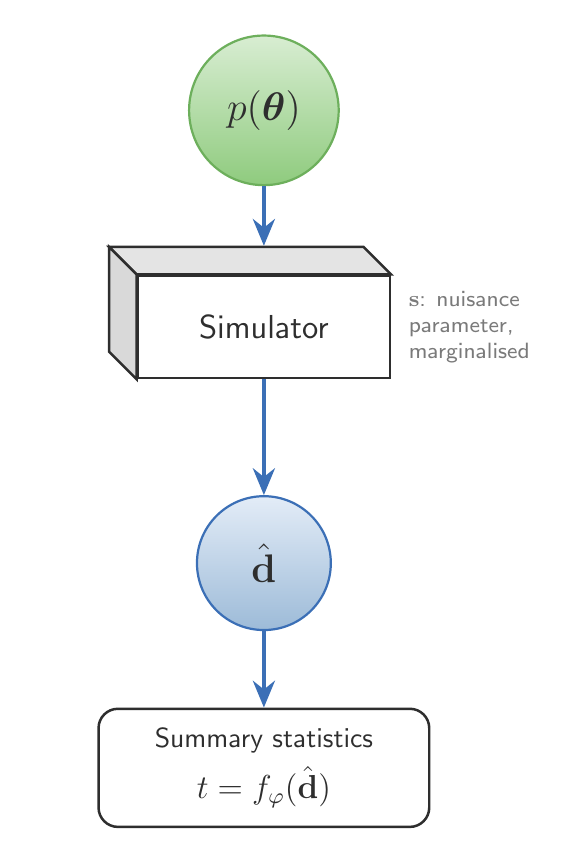
\begin{tikzpicture}
  \useasboundingbox (-3.0,-9.25) rectangle (3.75,1.05);

  \node[prior] (p) at (0,0) {$p(\boldsymbol\theta)$};

  \ifnum\stage=1
  % ---------------------------------------------------------------- implicit
  \simbox{sim}{(0,-2.75)}{3.2cm}{1.3cm}{Simulator}
  \node[font=\sffamily\footnotesize,text=greytx,align=left,anchor=west] at ($(sim.east)+(0.1,0)$)
       {$\mathbf{s}$: nuisance\\parameter,\\marginalised};
  \node[data] (map) at (0,-5.75) {$\hat{\mathbf{d}}$};
  \node[card,minimum width=4.2cm,minimum height=1.5cm] (sum) at (0,-8.35)
       {Summary statistics\\[4pt]\large$t = f_\varphi(\hat{\mathbf{d}})$};
  \draw[flowarr] (p) -- (sim.north |- 0,-1.72);
  \draw[flowarr] (sim) -- (map);
  \draw[flowarr] (map) -- (sum);
  \else
  % ---------------------------------------------------------------- explicit
  \node[diamond,draw=ink,line width=0.9pt,fill=white,minimum size=1.55cm,text=ink,font=\Large]
       (s) at (2.75,-3.35) {$\mathbf{s}$};
  \simbox{fm}{(0,-3.35)}{3.2cm}{1.45cm}{Forward model\\[2pt]$\mathcal{A}(\mathbf{s},\boldsymbol\theta)$}
  \node[data] (map) at (0,-6.25) {$\hat{\mathbf{d}}$};
  \node[card,minimum width=4.2cm,minimum height=1.5cm] (lik) at (0,-8.35)
       {compared with the data\\[4pt]\large$\lVert\hat{\mathbf{d}}-\mathbf{d}\rVert_2$};
  % straight down onto the top face, and s straight in from the side
  \draw[flowarr] (p.south) -- (p.south |- 0,{-3.35+0.725+0.35});
  \draw[flowarr] (s.west) -- (fm.east);
  \draw[flowarr] (fm) -- (map);
  \draw[flowarr] (map) -- (lik);
  \fi
\end{tikzpicture}
\end{document}
" (and explicit, \stage{2}), then pdftocairo -svg.
\documentclass[tikz,border=4pt]{standalone}
\usepackage{tikz}
\usepackage{amsmath}
\usepackage[T1]{fontenc}
\usetikzlibrary{arrows.meta,positioning,calc,shapes.geometric}

\providecommand{\stage}{1}

\definecolor{ink}{HTML}{2E2E2E}
\definecolor{greytx}{HTML}{7A7A7A}
\definecolor{flow}{HTML}{3B6FB6}
\definecolor{priortop}{HTML}{D8EDD2}
\definecolor{priorbot}{HTML}{8FCB7E}
\definecolor{priorrim}{HTML}{6DAF5C}
\definecolor{side}{HTML}{E4E4E4}
\definecolor{datatop}{HTML}{E3ECF7}
\definecolor{databot}{HTML}{9DBBD8}

\tikzset{
  prior/.style={circle,minimum size=1.9cm,draw=priorrim,line width=0.8pt,
                top color=priortop,bottom color=priorbot,text=ink,font=\Large},
  flowarr/.style={-{Stealth[length=3.4mm,width=2.8mm]},line width=1.5pt,draw=flow},
  data/.style={circle,minimum size=1.7cm,draw=flow,line width=0.8pt,
               top color=datatop,bottom color=databot,text=ink,font=\Large},
  card/.style={draw=ink,line width=0.9pt,rounded corners=7pt,fill=white,align=center,
               text=ink,font=\sffamily},
}

% A white 3D box: front face as a node, with a bevelled top and left side behind it.
% #1 node name, #2 position, #3 width, #4 height, #5 label
\newcommand{\simbox}[5]{%
  \node[draw=ink,line width=0.9pt,fill=white,minimum width=#3,minimum height=#4,
        align=center,text=ink,font=\sffamily\large] (#1) at #2 {#5};
  \fill[side,draw=ink,line width=0.9pt]
    (#1.north west) -- ++(-0.35,0.35) -- ($(#1.north east)+(-0.35,0.35)$) -- (#1.north east) -- cycle;
  \fill[side!70!black!40,draw=ink,line width=0.9pt]
    (#1.north west) -- ++(-0.35,0.35) -- ($(#1.south west)+(-0.35,0.35)$) -- (#1.south west) -- cycle;
}

\begin{document}
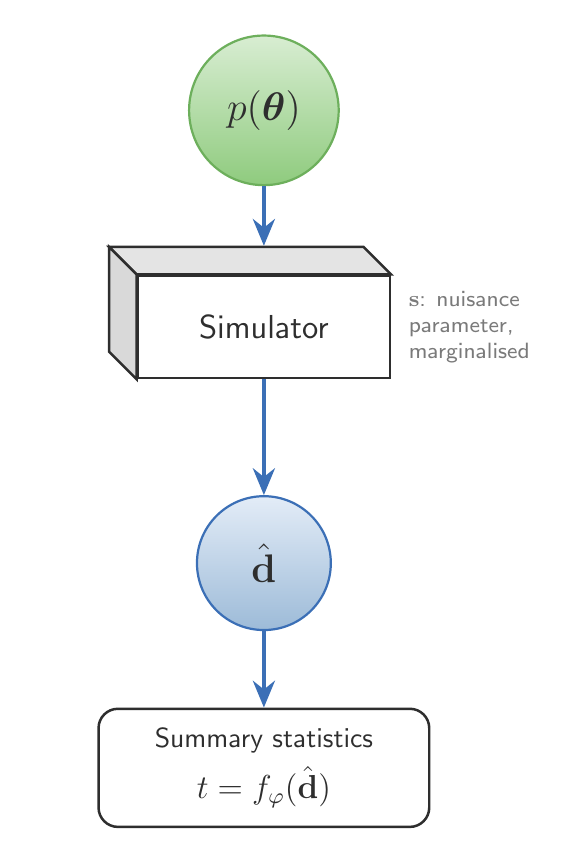
\begin{tikzpicture}
  \useasboundingbox (-3.0,-9.25) rectangle (3.75,1.05);

  \node[prior] (p) at (0,0) {$p(\boldsymbol\theta)$};

  \ifnum\stage=1
  % ---------------------------------------------------------------- implicit
  \simbox{sim}{(0,-2.75)}{3.2cm}{1.3cm}{Simulator}
  \node[font=\sffamily\footnotesize,text=greytx,align=left,anchor=west] at ($(sim.east)+(0.1,0)$)
       {$\mathbf{s}$: nuisance\\parameter,\\marginalised};
  \node[data] (map) at (0,-5.75) {$\hat{\mathbf{d}}$};
  \node[card,minimum width=4.2cm,minimum height=1.5cm] (sum) at (0,-8.35)
       {Summary statistics\\[4pt]\large$t = f_\varphi(\hat{\mathbf{d}})$};
  \draw[flowarr] (p) -- (sim.north |- 0,-1.72);
  \draw[flowarr] (sim) -- (map);
  \draw[flowarr] (map) -- (sum);
  \else
  % ---------------------------------------------------------------- explicit
  \node[diamond,draw=ink,line width=0.9pt,fill=white,minimum size=1.55cm,text=ink,font=\Large]
       (s) at (2.75,-3.35) {$\mathbf{s}$};
  \simbox{fm}{(0,-3.35)}{3.2cm}{1.45cm}{Forward model\\[2pt]$\mathcal{A}(\mathbf{s},\boldsymbol\theta)$}
  \node[data] (map) at (0,-6.25) {$\hat{\mathbf{d}}$};
  \node[card,minimum width=4.2cm,minimum height=1.5cm] (lik) at (0,-8.35)
       {compared with the data\\[4pt]\large$\lVert\hat{\mathbf{d}}-\mathbf{d}\rVert_2$};
  % straight down onto the top face, and s straight in from the side
  \draw[flowarr] (p.south) -- (p.south |- 0,{-3.35+0.725+0.35});
  \draw[flowarr] (s.west) -- (fm.east);
  \draw[flowarr] (fm) -- (map);
  \draw[flowarr] (map) -- (lik);
  \fi
\end{tikzpicture}
\end{document}
" (and explicit, \stage{2}), then pdftocairo -svg.
\documentclass[tikz,border=4pt]{standalone}
\usepackage{tikz}
\usepackage{amsmath}
\usepackage[T1]{fontenc}
\usetikzlibrary{arrows.meta,positioning,calc,shapes.geometric}

\providecommand{\stage}{1}

\definecolor{ink}{HTML}{2E2E2E}
\definecolor{greytx}{HTML}{7A7A7A}
\definecolor{flow}{HTML}{3B6FB6}
\definecolor{priortop}{HTML}{D8EDD2}
\definecolor{priorbot}{HTML}{8FCB7E}
\definecolor{priorrim}{HTML}{6DAF5C}
\definecolor{side}{HTML}{E4E4E4}
\definecolor{datatop}{HTML}{E3ECF7}
\definecolor{databot}{HTML}{9DBBD8}

\tikzset{
  prior/.style={circle,minimum size=1.9cm,draw=priorrim,line width=0.8pt,
                top color=priortop,bottom color=priorbot,text=ink,font=\Large},
  flowarr/.style={-{Stealth[length=3.4mm,width=2.8mm]},line width=1.5pt,draw=flow},
  data/.style={circle,minimum size=1.7cm,draw=flow,line width=0.8pt,
               top color=datatop,bottom color=databot,text=ink,font=\Large},
  card/.style={draw=ink,line width=0.9pt,rounded corners=7pt,fill=white,align=center,
               text=ink,font=\sffamily},
}

% A white 3D box: front face as a node, with a bevelled top and left side behind it.
% #1 node name, #2 position, #3 width, #4 height, #5 label
\newcommand{\simbox}[5]{%
  \node[draw=ink,line width=0.9pt,fill=white,minimum width=#3,minimum height=#4,
        align=center,text=ink,font=\sffamily\large] (#1) at #2 {#5};
  \fill[side,draw=ink,line width=0.9pt]
    (#1.north west) -- ++(-0.35,0.35) -- ($(#1.north east)+(-0.35,0.35)$) -- (#1.north east) -- cycle;
  \fill[side!70!black!40,draw=ink,line width=0.9pt]
    (#1.north west) -- ++(-0.35,0.35) -- ($(#1.south west)+(-0.35,0.35)$) -- (#1.south west) -- cycle;
}

\begin{document}
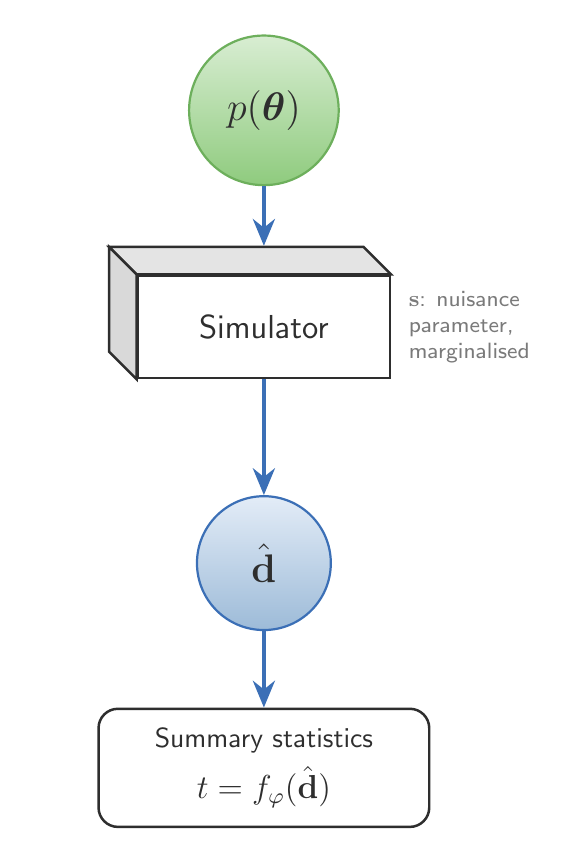
\begin{tikzpicture}
  \useasboundingbox (-3.0,-9.25) rectangle (3.75,1.05);

  \node[prior] (p) at (0,0) {$p(\boldsymbol\theta)$};

  \ifnum\stage=1
  % ---------------------------------------------------------------- implicit
  \simbox{sim}{(0,-2.75)}{3.2cm}{1.3cm}{Simulator}
  \node[font=\sffamily\footnotesize,text=greytx,align=left,anchor=west] at ($(sim.east)+(0.1,0)$)
       {$\mathbf{s}$: nuisance\\parameter,\\marginalised};
  \node[data] (map) at (0,-5.75) {$\hat{\mathbf{d}}$};
  \node[card,minimum width=4.2cm,minimum height=1.5cm] (sum) at (0,-8.35)
       {Summary statistics\\[4pt]\large$t = f_\varphi(\hat{\mathbf{d}})$};
  \draw[flowarr] (p) -- (sim.north |- 0,-1.72);
  \draw[flowarr] (sim) -- (map);
  \draw[flowarr] (map) -- (sum);
  \else
  % ---------------------------------------------------------------- explicit
  \node[diamond,draw=ink,line width=0.9pt,fill=white,minimum size=1.55cm,text=ink,font=\Large]
       (s) at (2.75,-3.35) {$\mathbf{s}$};
  \simbox{fm}{(0,-3.35)}{3.2cm}{1.45cm}{Forward model\\[2pt]$\mathcal{A}(\mathbf{s},\boldsymbol\theta)$}
  \node[data] (map) at (0,-6.25) {$\hat{\mathbf{d}}$};
  \node[card,minimum width=4.2cm,minimum height=1.5cm] (lik) at (0,-8.35)
       {compared with the data\\[4pt]\large$\lVert\hat{\mathbf{d}}-\mathbf{d}\rVert_2$};
  % straight down onto the top face, and s straight in from the side
  \draw[flowarr] (p.south) -- (p.south |- 0,{-3.35+0.725+0.35});
  \draw[flowarr] (s.west) -- (fm.east);
  \draw[flowarr] (fm) -- (map);
  \draw[flowarr] (map) -- (lik);
  \fi
\end{tikzpicture}
\end{document}
" (and explicit, \stage{2}), then pdftocairo -svg.
\documentclass[tikz,border=4pt]{standalone}
\usepackage{tikz}
\usepackage{amsmath}
\usepackage[T1]{fontenc}
\usetikzlibrary{arrows.meta,positioning,calc,shapes.geometric}

\providecommand{\stage}{1}

\definecolor{ink}{HTML}{2E2E2E}
\definecolor{greytx}{HTML}{7A7A7A}
\definecolor{flow}{HTML}{3B6FB6}
\definecolor{priortop}{HTML}{D8EDD2}
\definecolor{priorbot}{HTML}{8FCB7E}
\definecolor{priorrim}{HTML}{6DAF5C}
\definecolor{side}{HTML}{E4E4E4}
\definecolor{datatop}{HTML}{E3ECF7}
\definecolor{databot}{HTML}{9DBBD8}

\tikzset{
  prior/.style={circle,minimum size=1.9cm,draw=priorrim,line width=0.8pt,
                top color=priortop,bottom color=priorbot,text=ink,font=\Large},
  flowarr/.style={-{Stealth[length=3.4mm,width=2.8mm]},line width=1.5pt,draw=flow},
  data/.style={circle,minimum size=1.7cm,draw=flow,line width=0.8pt,
               top color=datatop,bottom color=databot,text=ink,font=\Large},
  card/.style={draw=ink,line width=0.9pt,rounded corners=7pt,fill=white,align=center,
               text=ink,font=\sffamily},
}

% A white 3D box: front face as a node, with a bevelled top and left side behind it.
% #1 node name, #2 position, #3 width, #4 height, #5 label
\newcommand{\simbox}[5]{%
  \node[draw=ink,line width=0.9pt,fill=white,minimum width=#3,minimum height=#4,
        align=center,text=ink,font=\sffamily\large] (#1) at #2 {#5};
  \fill[side,draw=ink,line width=0.9pt]
    (#1.north west) -- ++(-0.35,0.35) -- ($(#1.north east)+(-0.35,0.35)$) -- (#1.north east) -- cycle;
  \fill[side!70!black!40,draw=ink,line width=0.9pt]
    (#1.north west) -- ++(-0.35,0.35) -- ($(#1.south west)+(-0.35,0.35)$) -- (#1.south west) -- cycle;
}

\begin{document}
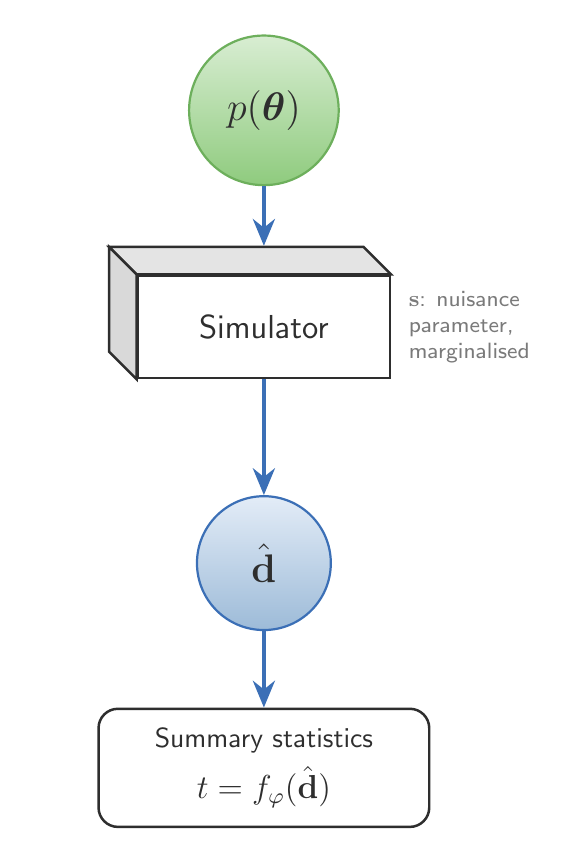
\begin{tikzpicture}
  \useasboundingbox (-3.0,-9.25) rectangle (3.75,1.05);

  \node[prior] (p) at (0,0) {$p(\boldsymbol\theta)$};

  \ifnum\stage=1
  % ---------------------------------------------------------------- implicit
  \simbox{sim}{(0,-2.75)}{3.2cm}{1.3cm}{Simulator}
  \node[font=\sffamily\footnotesize,text=greytx,align=left,anchor=west] at ($(sim.east)+(0.1,0)$)
       {$\mathbf{s}$: nuisance\\parameter,\\marginalised};
  \node[data] (map) at (0,-5.75) {$\hat{\mathbf{d}}$};
  \node[card,minimum width=4.2cm,minimum height=1.5cm] (sum) at (0,-8.35)
       {Summary statistics\\[4pt]\large$t = f_\varphi(\hat{\mathbf{d}})$};
  \draw[flowarr] (p) -- (sim.north |- 0,-1.72);
  \draw[flowarr] (sim) -- (map);
  \draw[flowarr] (map) -- (sum);
  \else
  % ---------------------------------------------------------------- explicit
  \node[diamond,draw=ink,line width=0.9pt,fill=white,minimum size=1.55cm,text=ink,font=\Large]
       (s) at (2.75,-3.35) {$\mathbf{s}$};
  \simbox{fm}{(0,-3.35)}{3.2cm}{1.45cm}{Forward model\\[2pt]$\mathcal{A}(\mathbf{s},\boldsymbol\theta)$}
  \node[data] (map) at (0,-6.25) {$\hat{\mathbf{d}}$};
  \node[card,minimum width=4.2cm,minimum height=1.5cm] (lik) at (0,-8.35)
       {compared with the data\\[4pt]\large$\lVert\hat{\mathbf{d}}-\mathbf{d}\rVert_2$};
  % straight down onto the top face, and s straight in from the side
  \draw[flowarr] (p.south) -- (p.south |- 0,{-3.35+0.725+0.35});
  \draw[flowarr] (s.west) -- (fm.east);
  \draw[flowarr] (fm) -- (map);
  \draw[flowarr] (map) -- (lik);
  \fi
\end{tikzpicture}
\end{document}
